\section{理論}
第\ref{sec:exp-system}節で示した通り,本研究の系では超音波照射された擬塑性流体中を球が落下する.はじめに,擬塑性流体中を球が落下する理論を示すことで,球の終端速度の理論式を得る.続いて,球の落下によるせん断速度より,球の落下による応力を見積もる.最後に,超音波照射された擬塑性流体中を落下する球の高速化のメカニズムを考察し,高速化の理論式を見積もる.

\subsection{擬塑性流体中における球の落下}
本研究の系において,代表速度,代表長さとして,落下球の終端速度$U_\text{T}$,球直径$D=2a$を選ぶ.Power-law model (式(\ref{eq:power-low}))が適用できる流体中おける粒子レイノルズ数は次式で表される\cite{ref:1,ref:8-5}.
\begin{eqnarray}
    Re = \frac{\rho_1 \left(2a\right)^n U_T^{2-n}}{k} .
    \label{eq:re}
\end{eqnarray}
ここで,$\rho_1$は溶液密度である.今回の実験結果の代表例(鋼球,直径10mm,PAA1.0wt.\%)において,溶液密度$\rho_1\approx$1000kg/m$^3$,$2a=$0.01m,$U_T \approx$0.2m/s,$k=$8.8Pa$\cdot \text{s}^n$,$n=$0.23である.この条件を,式(\ref{eq:re})に代入すると$Re\approx$2.3と概算できる.粒子周囲の流れは慣性に比べて粘性が支配的であり,ストークス方程式に概ね従うものと考える.

超音波の伝播に関して,音波の圧力変動の時間スケールは$O\left(10^{-5}\right)$sである.これは,球の落下現象の時間スケール $O\left(10^{0}\right)$sと比べて非常に短い.球の落下に関しては,落下時間スケールで粗視化した平均的な挙動に着目する.球周囲に存在する非圧縮性流体の運動量輸送を考える.球によって誘起される応力テンソルを$\bm{\sigma}$,流体の密度を$\rho$,周囲流体の速度ベクトルを$\bm{v}$,体積力を$\bm{X}$とすると,
\begin{eqnarray}
    \rho \frac{D\bm{v}}{Dt} = \bm{X} + \nabla \cdot \bm{\sigma} ,
    \label{eq:undou}
\end{eqnarray}
となる.また,非圧縮性流体を仮定しているため,以下の連続の式が成り立つ.
\begin{eqnarray}
    \nabla \cdot \bm{v} = 0 .
    \label{eq:renzoku}
\end{eqnarray}
粒子重心位置から見た移動座標系では,式(\ref{eq:undou})の左辺は,以下のように書ける.
\begin{eqnarray}
    \frac{D\bm{v}}{Dt} = \frac{\partial \bm{v}}{\partial t} + \left(\bm{v} - \bm{U}_T \cdot \nabla \right) \bm{v} .
    \label{eq:nabie}
\end{eqnarray}
流れは十分に発達し,定常状態であると仮定すると,式(\ref{eq:nabie})の右辺第1項の時間微分項は0となる.低レイノルズ数であることからStokes近似を用いると,式(\ref{eq:nabie})の右辺第2項の慣性項は無視できる.加えて,粒子周囲流体には密度差がないため,静水圧分を除いた圧力を使って応力${\bm \sigma}$と書くと,体積力${\bm X}$は0と書ける.これらの仮定より,式(\ref{eq:undou})を以下のように簡略化する.
\begin{eqnarray}
    \nabla \cdot \bm{\sigma} = 0 .
    \label{eq:sigma-}
\end{eqnarray}

粒子重心周りの球形領域において,ガウスの発散定理を適用すると以下の関係が成り立つ.
\begin{eqnarray}
    \int_S{\bm{\sigma \cdot \bm{n}}}dS = \int_V{\nabla \cdot \bm{\sigma}}dV ,
    \label{eq:gaussian}
\end{eqnarray}
ここで,$\bm{n}$は球領域および粒子の表面での外向き単位法線ベクトル,$S$はそれぞれの球の表面積,$V$は2つの球の間の体積を表す.式(\ref{eq:sigma-})より,式(\ref{eq:gaussian})の右辺は0とする.式(\ref{eq:sigma-}),(\ref{eq:gaussian})は任意の流体体積に関して成り立つため,球の表面($r = a$)と球外部の任意の領域($r > a$)において,以下の関係が成り立つ.
\begin{eqnarray}
    \int_{r=a}\bm{\sigma}\cdot\bm{e}_r dS=\int_r\bm{\sigma}\cdot\bm{e}_r dS .
    \label{eq:inte}
\end{eqnarray}
ここで,球領域表面では$\bm{n} = \bm{e}_r$,粒子表面では$\bm{n}=-\bm{e}_r$である.式(\ref{eq:inte})は,任意の領域での,面積力の釣り合いを表す.$r = a$における時間平均応力のオーダーを$\langle\sigma\rangle_a$,$r$における時間平均応力のオーダーを$\langle\sigma\rangle_r$とそれぞれする.球の表面積は$S=4\pi r^2$であるので,式(\ref{eq:inte})より,以下の関係が成り立つとみなす.
\begin{eqnarray}
    4\pi a^2\langle\sigma\rangle_a \sim 4\pi r^2\langle\sigma\rangle_r .
    \label{eq:sigma1}
\end{eqnarray}
粒子表面での表面力と体積力の釣り合いより,以下の関係を考える.
\begin{eqnarray}
    4\pi a^2\langle\sigma\rangle_a = \frac{4}{3} \pi a^3 \Delta \rho g .
    \label{eq:sigma2}
\end{eqnarray}
となる.ここで,$\Delta \rho$は球と流体の密度差,$g$は重力加速度である.式(\ref{eq:sigma1}),(\ref{eq:sigma2})より,以下のようにオーダー評価できる.
\begin{eqnarray}
    \langle\sigma\rangle_r \sim \frac{a^3\Delta\rho g}{3r^2} .
\end{eqnarray}
低レイノルズ数で粘性項が支配的であることから,応力を以下のように概算する.
\begin{eqnarray}
    \langle\sigma\rangle_r \sim \mu \dot{\gamma} .
    \label{eq:sigma3}
\end{eqnarray}
Power-law model(式(\ref{eq:power-low}))の粘度を式(\ref{eq:sigma3})に代入して整理すると以下の関係を得る.
\begin{eqnarray}
    \dot{\gamma} \sim \left(\frac{a^3\Delta\rho g}{3r^2 k}\right)^{\frac{1}{n}} ,
    \label{eq:gamma_abs}
\end{eqnarray}
次に,エネルギー散逸に関して考える.単位時間あたりのエネルギーバランスは,位置エネルギーと粘性によるエネルギー散逸の時間変化の釣り合いとして書ける.すなわち,
釣り合うため,より,以下の式が成立する.
\begin{eqnarray}
    \int_{r>a}\bar{\epsilon}dV = 4 \pi \int^\infty_a \bar{\epsilon}r^2 dr = \frac{4}{3}\pi a^3\Delta\rho g U_T ,
    \label{eq:eg}
\end{eqnarray}
と表される.ここで,$U_T$は球の終端速度,$\bar{\epsilon}$は時間平均された単位体積当たりのエネルギー散逸率である.また,エネルギー散逸率$\bar{\epsilon}$は,以下の様に概算される.
\begin{eqnarray}
    \bar{\epsilon} \sim \langle\sigma\rangle_r\dot{\gamma} \sim \mu \dot{\gamma}^2 \sim \frac{\langle\sigma\rangle_r^2}{\mu} .
    \label{eq:eps}
\end{eqnarray}
式(\ref{eq:sigma3}),(\ref{eq:eg}),(\ref{eq:eps})より,超音波照射されていないときの終端速度$U_\text{off}$は
\begin{eqnarray}
    U_\text{off} \sim \frac{a^3\Delta\rho g}{3}\int_a^\infty\frac{dr}{\mu r^2} ,
    \label{eq:UT0}
\end{eqnarray}
と見積もられる.式(\ref{eq:power-low}),(\ref{eq:gamma_abs}),(\ref{eq:UT0})より,終端速度は下記の様に書き直される.
\begin{eqnarray}
    U_\text{off} \sim \frac{a^3\Delta\rho g}{3}  \int^{\infty}_{a} \frac{dr}{\mu r^2} \sim \left(\frac{\Delta \rho g}{3k}\right)^{\frac{1}{n}}\frac{n}{2-n}a^{\frac{n+1}{n}} .
    \label{eq:UT}
\end{eqnarray}

\subsection{擬塑性流体中における球の落下による応力}
超音波照射された擬塑性流体中を落下する球の周囲流体をFig\ref{fig:layer}に示す.球の周囲より音響境界層,落下球による領域,バルク領域と分類される.

球の落下が影響を及ぼす領域において,$\dot{\gamma}$は,球の終端速度$U_\text{T}$と半径$a$を用いて,
\begin{eqnarray}
    \dot{\gamma} \sim \frac{U_\text{T}}{a},
    \label{eq:UTgamma}
\end{eqnarray}
と見積もられる.球の落下による粘度$\mu_\text{U}$は,式(\ref{eq:power-low})のPower-law modelより,
\begin{eqnarray}
    \mu_\text{U} \sim k \left(\frac{U_\text{T}}{a}\right)^{n-1} ,
    \label{eq:muU}
\end{eqnarray}
と見積もることができる.これより,式(\ref{eq:sigma3})より球の落下による応力$\tau_\text{U}$は,
\begin{eqnarray}
    \tau_\text{U} \sim k \left(\frac{U_\text{T}}{a}\right)^n ,
    \label{eq:tauU}
\end{eqnarray}
と見積もられる.

\begin{figure}[ht]
    \centering
    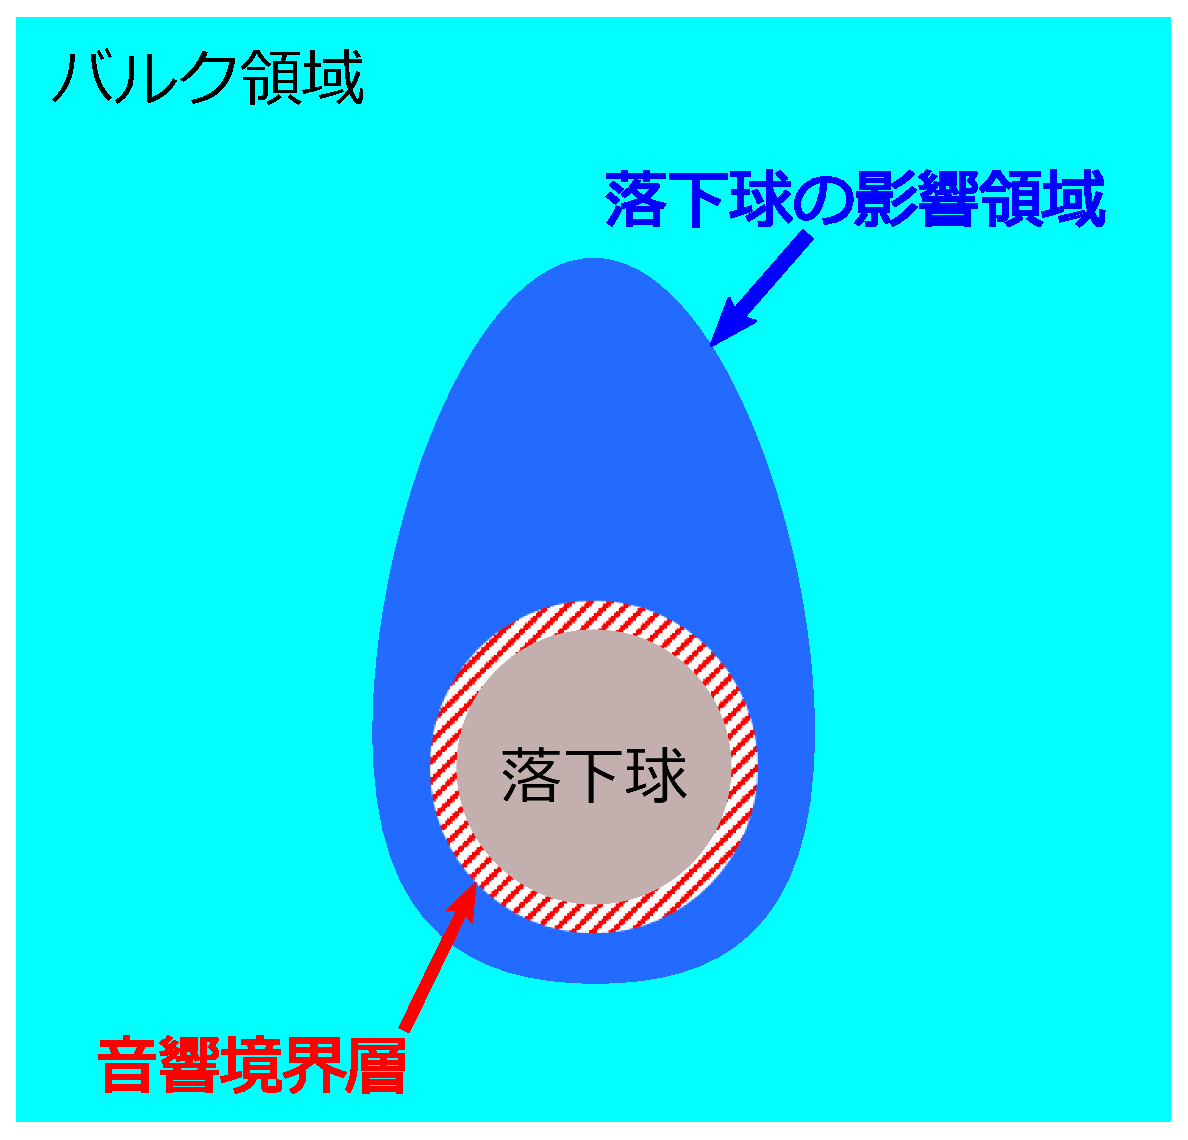
\includegraphics[width=0.5\textwidth]{4-Theory/boundary_layer.eps}
    \caption{Layers of the effect of a falling sphere on the fluid.}
    \label{fig:layer}
\end{figure}

\subsection{超音波照射に伴う球の高速化}
\label{sec:UTdiff}
超音波照射された本研究の系における,落下球の高速化に関して考える.音響境界層における,せん断速度の代表値は次のように概算される.
\begin{eqnarray}
    \dot{\gamma} \sim \frac{u}{\delta} .
    \label{eq:abl-delta}
\end{eqnarray}
ここで,$u$は音波によって加振される流体粒子速度,$\delta$は音響境界層厚さを表す.

流体粒子速度$u$に関して,球の落下方向を$z$とすると運動方程式は次式となる.
\begin{eqnarray}
    \frac{\partial u}{\partial t} + \frac{1}{\rho_1}\frac{\partial P}{\partial z} = 0 .
    \label{eq:newton-1}
\end{eqnarray}
ここで,$t$は時刻,$P$は圧力である.また,連続の式は圧縮性流体と仮定すると以下の式となる.
\begin{eqnarray}
    \frac{\partial u}{\partial z} + \frac{1}{\rho_1 c^2}\frac{\partial P}{\partial t} = 0 .
\end{eqnarray}
音波の周波数は一定であり,容器内の圧力変化は音波に依存するので,以下の近似を用いる.
\begin{eqnarray}
    \frac{\partial u}{\partial t} &\sim& uf ,\label{eq:1-1}\\
    \partial P &\sim& \Delta P ,\label{eq:1-2}\\
    \partial z &\sim& \lambda .\label{eq:1-3}
\end{eqnarray}
ここで,$\Delta P$は音響圧振動,$\lambda$は超音波の波長である.式(\ref{eq:1-1}),(\ref{eq:1-2}),(\ref{eq:1-3})を用いて,式(\ref{eq:newton-1})の近似を行うと次式のようになる.
\begin{eqnarray}
    uf \sim \frac{\Delta P}{\rho_1 \lambda} .
    \label{eq:u-1}
\end{eqnarray}
周波数$f$,波長$\lambda$,音速$c$の関係から式(\ref{eq:u-1})を書き換えると次式となる.
\begin{eqnarray}
    u \sim \frac{\Delta P}{\rho_1 c} .
\end{eqnarray}

式(\ref{eq:abl-delta})より,Power-law model(式(\ref{eq:power-low}))を適用すると,音響境界層における粘度$\mu_\text{ABL}$は次式の様に見積もられる.
\begin{eqnarray}
    \mu_\text{ABL} \sim k\left(\frac{u}{\delta}\right)^{n-1} ,
    \label{eq:muABL}
\end{eqnarray}
よって,音響境界層厚さ$\delta$は,
\begin{eqnarray}
    \delta \sim \sqrt{\frac{\mu_{ABL}}{\pi \rho_h f}} ,
    \label{eq:delta2}
\end{eqnarray}
と見積もられる\cite{deshpande2001vibrational,wiklund2012acoustofluidics}.ここで,周波数$f$である.よって,式(\ref{eq:delta2})を式(\ref{eq:muABL})に代入すると,次のように表される.
\begin{eqnarray}
    \delta \sim \left(\frac{k\left(\Delta P\right)^{n-1}}{\pi \rho^n_1 c^{n-1} f}\right)^{\frac{1}{n+1}} .
    \label{eq:delta}
\end{eqnarray}
ここで,音速$c$である.音響境界層粘度$\mu_{ABL}$とすると超音波照射下における終端速度$U_\text{on}$は,式(\ref{eq:UT})より,
\begin{eqnarray}
    U_\text{on} \sim \frac{a^3\Delta\rho g}{3}  \int^{\infty}_{a} \frac{dr}{\mu_{ABL} r^2} \sim \frac{a\Delta \rho \delta g}{3\mu_{ABL}} ,
    \label{eq:U_ABL}
\end{eqnarray}
と見積もられる.終端速度$U_T$における,粘度$\mu_U$とする.式(\ref{eq:UT}),(\ref{eq:U_ABL})より,超音波照射の有無による終端速度比は,
\begin{eqnarray}
    \frac{U_\text{on}}{U_\text{off}} \sim \frac{\mu_U}{\mu_{ABL}}\frac{\delta}{a} ,
    \label{eq:Udiff}
\end{eqnarray}
と表される.
